\section{Auswertung}
\label{sec:Auswertung}
\subsection{Bestimmung der Zeitkonstante durch die Entladung eines Kondensators}
Es wurde eine Entladekurve des Kondensators durch das Oszilloskop aufgenommen, die
in Abbildung \ref{fig:entladekurve} zu sehen ist.
\begin{figure}
  \centering
  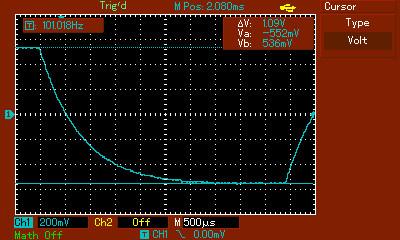
\includegraphics[width=250pt]{data/4a_volt.png}
  \caption{Entladekurve des Kondensators}
  \label{fig:entladekurve}
\end{figure}

Die daraus entnommenen Wertepaare sind in Tabelle \ref{tab:entladung} zu finden.

\begin{table}
\centering
\caption{Messdaten zur Entladung des Kondensators über den Widerstand}
\label{tab:entladung}
\begin{tabular}{c c}
\toprule
$U_\text{C}(t)/$mV & $t/$ms \\
\midrule
1088 &  0   \\
 560 &  0.5 \\
 304 &  1   \\
 152 &  1.5 \\
 80  &  2   \\
 36  &  2.5 \\
  8  &  3   \\
  4  &  3.5 \\
  2  &  4   \\
\bottomrule
\end{tabular}
\end{table}
Die anliegende Generatorspannung $U_0$ ist hierbei näherungsweise der Spannungsabfall
am Kondensator $U_\text{C}(0)$, da der betrachtete Zeitraum hinreichend lang ist, um von einer
fast vollständigen Entladung auszugehen.
Nach Teilen durch $U_\text{C}(0)$ und Logarithmieren von \eqref{eqn:kondensatorurelax}
folgt\footnote{Entgegen der Versuchsanleitung wird eine lineare Ausgleichsrechnug mit bezüglich
$U_\text{C}(0)$ normierten Spannungswerten durchgeführt, da es nicht möglich ist,
dimensionsbehaftete Größen zu logarithmieren.}

\begin{equation}
  \ln{\left(\frac{U_\mathrm{C}(t)}{U_0}\right)} = -\frac{t}{\tau}\,.
\end{equation}
Die graphische Darstellung der Messwerte und die Ausgleichsgerade ist in Abbildung \ref{fig:entladung}
zu sehen.
\begin{figure}
  \centering
  \includegraphics{build/uc.pdf}
  \caption{Auftragung von $\ln{\left(\frac{U_\mathrm{C}}{U_0}\right)}$ gegen $t$ und Graph der Ausgleichsfunktion}
  \label{fig:entladung}
\end{figure}
Die Ausgleichsgerade folgt allgemein \eqref{eqn:gerade}, sodass die Steigung der
Ausgleichsgerade $a$ mit der Zeitkonstanten $\tau$ des RC-Gliedes in dem Zusammenhang
$a = -1/\tau$ steht. Hier lässt sich $a$ zu
\begin{align}
  a = \SI{-1.62(007)}{\per\milli\second}
\end{align}
berechnen und für die nach dem ersten Messverfahren ermittelte Zeitkonstante
\footnote{Es gilt hierbei die Konvention, dass in allgemeinen Formeln \tau ohne
Index notiert wird. Wird die Ausgleichsrechnung durchgeführt und der Parameter
konkret ermittelt, wird er durchnummeriert.}
folgt dann
\begin{align}
\tau_1 = \SI{0.616(0027)}{\milli\second}\,.
\end{align}
Dabei beträgt die relative Unsicherheit 4.38\%.
\subsection{Bestimmung der Zeitkonstante durch Beachtung von Frequenzabhängigkeiten}

Die Messdaten für die eingestellte Frequenz $f$, die Kondensatorspannung
$U_\text{C}$ und die Differenz $a$ zwischen den Nulldurchgängen von Generatorspannung
und Kondensatorspannung können Tabelle \ref{tab:frequenzen} entnommen werden. Es wurde auch bereits
die Phasenverschiebung $\phi$ aus $a$ und $f$ mithilfe von \eqref{eqn:ab2phi} berechnet.

\begin{table}
\centering
\caption{Messdaten zur Frequenzabhängigkeit der Kondensatorspannung und der Phasenverschiebung}
\label{tab:frequenzen}
\begin{tabular}{c c c c}
\toprule
$f/Hz$ & $U_\text{C}(f)/$mV & $a/$ms & $\phi/$grad\\
\midrule
  20	&  492.30  &  1.12  &   8.06 \\
  30	&  490.85  &  1.00  &  10.80 \\
  40	&  487.05  &  0.92  &  13.25 \\
  50	&  482.15  &  0.80  &  14.40 \\
  60	&  475.17  &  0.78  &  16.85 \\
  70	&  469.05  &  0.78  &  19.56 \\
  80	&  461.20  &  0.76  &  21.89 \\
  90	&  452.80  &  0.75  &  24.36 \\
 100	&  442.15  &  0.74  &  26.78 \\
 150	&  393.80  &  0.68  &  36.72 \\
 200	&  347.30  &  0.62  &  44.93 \\
 300	&  273.00  &  0.54  &  57.89 \\
 400	&  220.20  &  0.46  &  65.66 \\
 500	&  183.00  &  0.38  &  68.40 \\
 600	&  155.70  &  0.33  &  71.71 \\
 700	&  135.60  &  0.3   &  74.59 \\
 800	&  119.80  &  0.27  &  77.18 \\
 900	&  107.30  &  0.24  &  77.76 \\
1000	&   97.00  &  0.22  &  79.20 \\
1500	&   65.50  &  0.15  &  83.16 \\
2000	&   49.35  &  0.12  &  84.96 \\
3000	&   33.06  &  0.08  &  86.40 \\
4000	&   24.88  &  0.06  &  86.40 \\
5000	&   19.96  &  0.05  &  89.28 \\
\bottomrule
\end{tabular}
\end{table}

\subsubsection{Analyse der Frequenzabhängigkeit der Kondensatorspannung}

Nach \eqref{eqn:kondensatorfrequenz} ist die Amplitude der Kondensatorspannung
$A(f)$ frequenzabhängig. Es wird eine nicht lineare Ausgleichsrechnung
einer normierten Amplitude $A(f)/U_0$ mit der frequenzunabhängigen Generatorspannung $U_0$
durchgeführt. Stets ist für die Kreisfrequenz $\omega = 2πf$ zu beachten.
Dabei gilt für die Ausgleichsfunktion
\begin{align}
  \frac{A(f)}{U_0} = \frac{1}{\sqrt{1+(2πdf)^2}}\,,
\end{align}
wobei für den Parameter $d = \tau$ gilt.
Die Auftragung der Messwerte aus Tabelle \ref{tab:frequenzen} und der Graph der Ausgleichsfunktion ist in Abbildung \ref{fig:amplitude}
zu sehen. Die f-Achse ist logarithmisch skaliert.

\begin{figure}
  \centering
  \includegraphics{build/amplitude.pdf}
  \caption{Auftragung von $A(f)/U_0$ gegen $f$ und Graph der Ausgleichsfunktion}
  \label{fig:amplitude}
\end{figure}

Für die konkrete zu den Messwerten gehörige Ausgleichsfunktion ergibt sich für den Wert der Zeitkonstanten mit dem zweiten Verfahren
\begin{align}
  d = \tau_2 = \SI{0.829(0006)}{\milli\second}\,
\end{align}
mit einer relativen Unsicherheit von 0.72\%.

\subsubsection{Analyse der Frequenzabhängigkeit der Phasenverschiebung}

Auch die Phasenverschiebung zwischen Kondensatorspannung und Generatorspannung $phi$
ist frequenzabhängig, wie an \eqref{eqn:phasenfrequenz} ersichtlich ist.
Erneut wird eine Ausgleichsrechnung für die Messwerte aus Tabelle \ref{tab:frequenzen}
durchgeführt. Die Ausgleichsfunktion ist hierbei
\begin{align}
  \phi(f) = \arctan(2πef)\,.
\end{align}
Dabei ist der Parameter $e = \tau$. Die Messwerte und der Graph der Ausgleichsfunktion finden sich
in Abbildung \ref{fig:phiplot}.

\begin{figure}
  \centering
  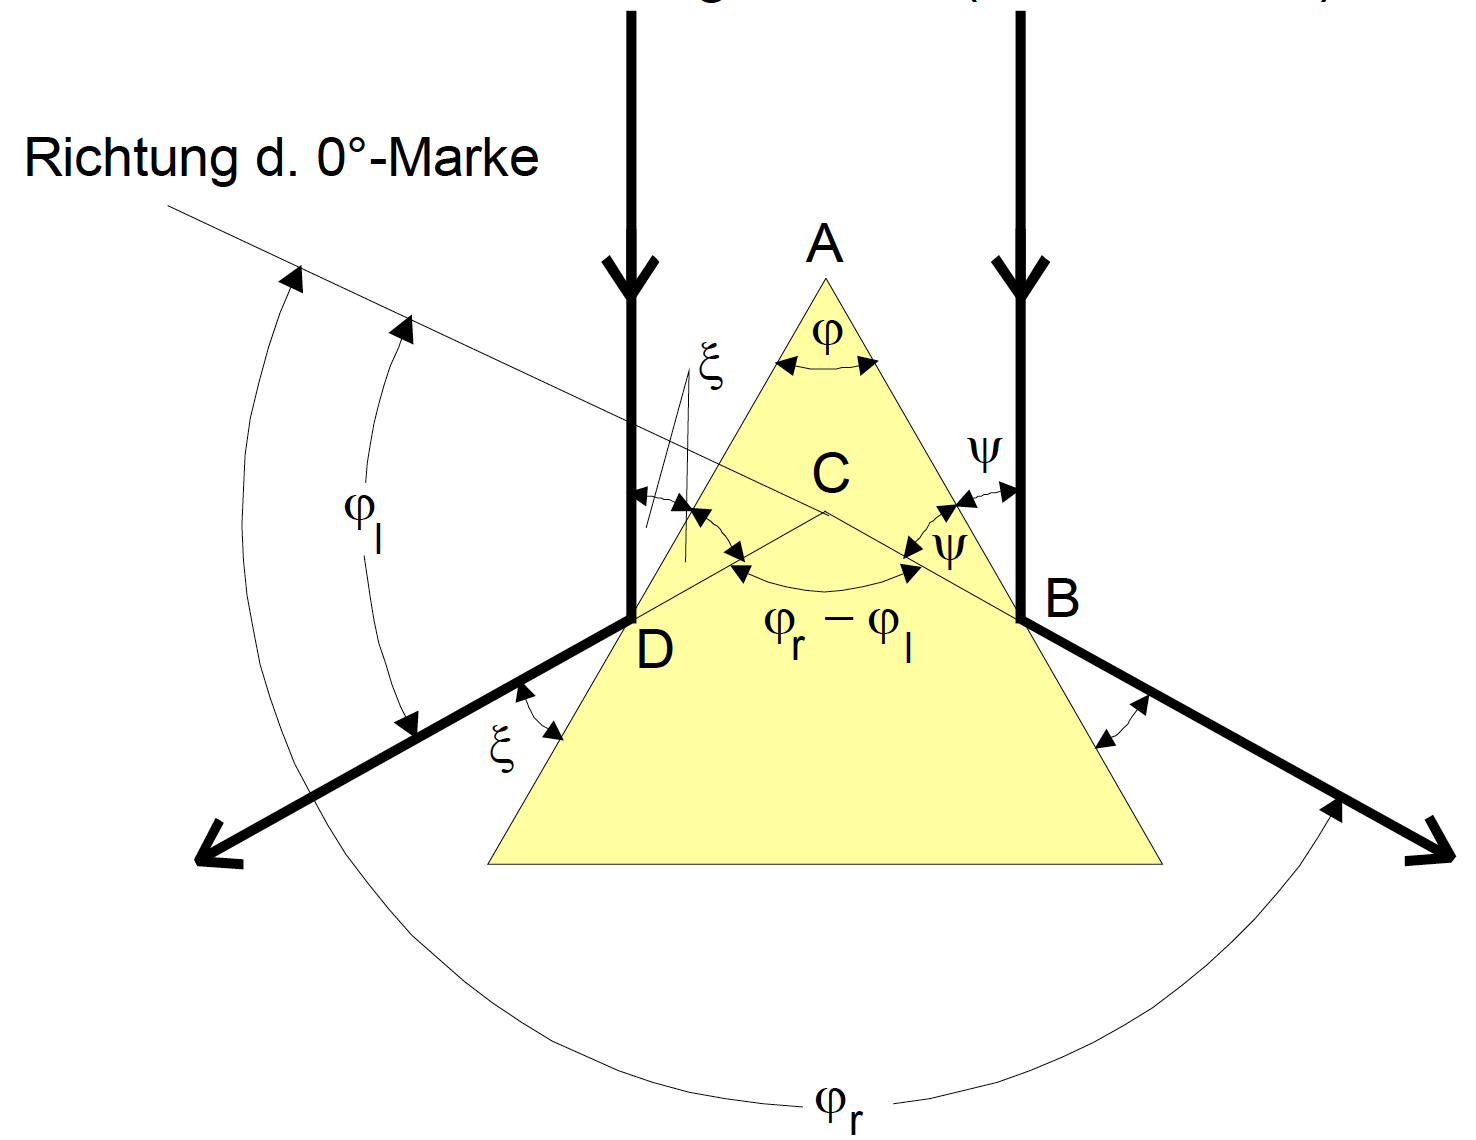
\includegraphics{build/phi.pdf}
  \caption{Auftragung von $\phi(f)$ gegen $f$ und Graph der Ausgleichsfunktion}
  \label{fig:phiplot}
\end{figure}

Der Parameter der Ausgleichsfunktion und damit auch der Wert für die
Zeitkonstante gemäß des dritten Verfahrens ergibt sich hier zu
\begin{align}
  e = \tau_3 = \SI{0.822(0010)}{\milli\second}\,
\end{align}
mit einer relativen Unsicherheit von 1,22\%.

Nun wird der Zusammenhang zwischen der Amplitude der Kondensatorspannung und der Phasenverschiebung betrachtet.
Es kann \eqref{eqn:phasenfrequenz} umgestellt werden zu zu
\begin{align}
  \frac{\sin(\phi)}{\cos(\phi)} = -ω\tau\,.
\end{align}
Wird dieses Ergebnis in \eqref{eqn:amplitude} eingesetzt, so ergibt sich für die Abhängigkeit der normierten
Amplitude $A(\phi)/U_0$ von der Phasenverschiebung $\phi$ der Zusammenhang
\begin{align}
  \frac{A(\phi)}{U_0} = \cos(\phi)\,.
\end{align}
Dieser wird hier für die vorliegenden Messwerte in Abbildung \ref{fig:polarplot} in einem
Polarkoordinatensystem veranschaulicht. Die Theoriekurve ist ebenso eingezeichnet.

\begin{figure}[H]
  \centering
  \includegraphics{build/polar.pdf}
  \caption{Veranschaulichung der Abhängigkeit der normierten Amplitude $A(\phi)/U_0$ von der gemessenen Phasenverschiebung}
  \label{fig:polarplot}
\end{figure}

\subsection{Der RC-Kreis als Integrator}

Für hohe angelegte Frequenzen sollte der RC-Kreis die angelegte Spannung integrieren.
Das bedeutet, dass der Graph der am Kondensator gemessenen Spannung dem Graphen der
Stammfunktion der angelegten Generatorspannung entsprechen sollte. In diesem Versuchsteil
wurde für alle angelegten Spannungen die Frequenz $f=191.8$ kHz gewählt.
Die erste an den RC-Kreis angelegte Spannung ist eine Reckteckspannung. Die Stammfunktion
zu dieser sollte gleichmäßig ansteigende Flanken dort haben, wo die Rechteckspannung
positiv ist und gleichmäßig abfallende Flanken dort, wo die Rechteckspannung
negativ ist. Es gilt der Zusammenhang
\begin{align}
  f(x)&=
  \begin{cases}
    c & 0<x\leq a\\
    -c & a<x\leq 2a
  \end{cases}
  & F(x)&=
  \begin{cases}
    c x & 0<x\leq a\\
    -c x & a<x\leq 2a
  \end{cases}
\end{align}
Genau dieses Verhalten ist in \ref{fig:rechteck} zu sehen. Der blaue Graph beschreibt
dabei die an das RC-Glied angelegte Spannung und der gelbe Graph die am Kondensator
abgegriffene Spannung.
\begin{figure}
  \centering
  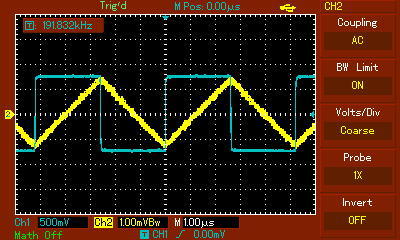
\includegraphics[width=250pt]{data/integration_rechteck.PNG}
  \caption{Graphen der Generatorspannung und der Spannung am Kondensator bei anglegter
  Rechteckspannung}
  \label{fig:rechteck}
\end{figure}


Wird an das RC-Glied eine Sägezahnspannung angelegt, so sollte die am Kondensator
abgegriffene Spannung eine sich periodisch wiederholende Funktion beschreiben, die
Extrema an den Nullstellen sowie Wendepunkten an den Extrema des Graphen der
Generatorspannung besitzt. Es gilt
\begin{align}
  f(x)&=
  \begin{cases}
    c x & -a<x\leq a\\
    -c x & a<x\leq 3a
  \end{cases}
  & F(x)&=
  \begin{cases}
    \frac{c}{2} x^2 & -a<x\leq a\\
    -\frac{c}{2} x^2 & a<x\leq 3a
  \end{cases}
\end{align}
Die Graphen der Messung \ref{fig:saegezahn} erfüllen diesen Zusammenhang.
Der blaue Graph beschreibt erneut den Verlauf der angelegten Generatorspannung und
der gelbe Graph den Verlauf der am Kondensator abgegriffenen Spannung.
\begin{figure}
  \centering
  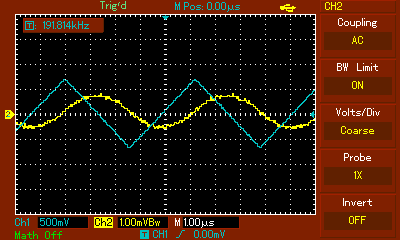
\includegraphics[width=250pt]{data/integration_saegezahn.PNG}
  \caption{Graphen der Generatorspannung und der Spannung am Kondensator bei anglegter
  Sägezahnspannung}
  \label{fig:saegezahn}
\end{figure}


Wird an den RC-Kreis eine sinusförmige Spannung angelegt, so sollte sich nach bei der
Integration gemäß
\begin{equation}
  \int c\sin(t) \, \symup{d}t=-c\cos(t)
\end{equation}
eine Spannung ergeben, die dem Graphen von $-\cos(t)$ entspricht. Der Verlauf der
im Versuch aufgenommenen Graphen \ref{fig:sinus} folgt dieser Beziehung mit $D = 0$. Hier beschreibt der blaue Graph
wieder den Verlauf der angelegten Generatorspannung und der gelbe Graph den Verlauf der
am Kondensator abgegriffenen Spannung.
\begin{figure}
  \centering
  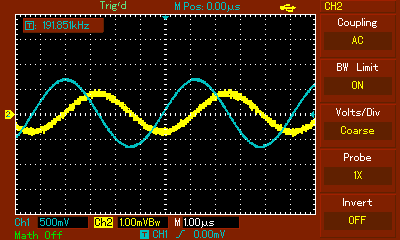
\includegraphics[width=250pt]{data/integration_sinus.PNG}
  \caption{Graphen der Generatorspannung und der Spannung am Kondensator bei anglegter
  Sinusspannung}
  \label{fig:sinus}
\end{figure}
